\documentclass[11pt]{article}
\usepackage[margin=1in]{geometry}
\usepackage[T1]{fontenc}
\usepackage[utf8]{inputenc}
\usepackage{booktabs}
\usepackage{longtable}
\usepackage{array}
\usepackage{amsmath}
\usepackage{amssymb}
\usepackage{hyperref}
\usepackage{float}
\usepackage{tikz}
\usetikzlibrary{positioning,arrows.meta}

\title{Fine-Tuning Report: TokenFusionAVTCA on RAVDESS}
\author{Emotion-Detect Repository}
\date{May 7, 2026}

\begin{document}
\maketitle

\section{Executive Summary}
This report documents the latest fine-tuning run of the shared-token multimodal architecture (\texttt{TokenFusionAVTCA}) and compares it to the previous model behavior. The previous system showed class collapse and weak minority-class boundaries. The new system demonstrates a strong increase in class balance and macro F1 on the reported validation checkpoints.

\section{Run Context}
\subsection{Training Command Used}
\begin{verbatim}
CUDA_VISIBLE_DEVICES=0,1 python main.py \
  --model token_fusion_avtca \
  --num_heads 4 \
  --embed_dim 256 \
  --transformer_depth 4 \
  --fusion_tokens 4 \
  --token_grid 4 \
  --dropout 0.2 \
  --attention_dropout 0.1 \
  --optimizer adamw \
  --learning_rate 1e-4 \
  --weight_decay 1e-2 \
  --use_class_weights true \
  --label_smoothing 0.05 \
  --batch_size 16 \
  --n_epochs 80 \
  --seed 42 \
  --use_amp true
\end{verbatim}

\subsection{Hardware and Parallelism}
\begin{itemize}
  \item Multi-GPU run with two CUDA devices (\texttt{CUDA\_VISIBLE\_DEVICES=0,1}).
  \item Model path updated to use \texttt{DataParallel} when multiple GPUs are visible.
\end{itemize}

\section{Current Code Design}
The current implementation uses one shared multimodal transformer, not two separate modality branches. The design in code follows:
\begin{itemize}
  \item \textbf{Audio tokenizer}: Conv1D stem + projection to audio tokens.
  \item \textbf{Video tokenizer}: Conv2D stem + channel/spatial/local refinement + projection to video tokens.
  \item \textbf{Fusion sequence}: \([CLS]\) + learned fusion tokens + audio tokens + video tokens.
  \item \textbf{Token identity}: learned modality embeddings and learned positional embeddings.
  \item \textbf{Shared encoder}: one transformer encoder stack over the full fused sequence.
  \item \textbf{Classifier}: uses fused representations only (CLS, fusion-token summary, pooled token context).
\end{itemize}

This design directly addresses the prior late-fusion weakness by forcing token-level audio-video interaction before classification.

\subsection{Architecture Diagram (Vertical)}
\begin{figure}[H]
\centering
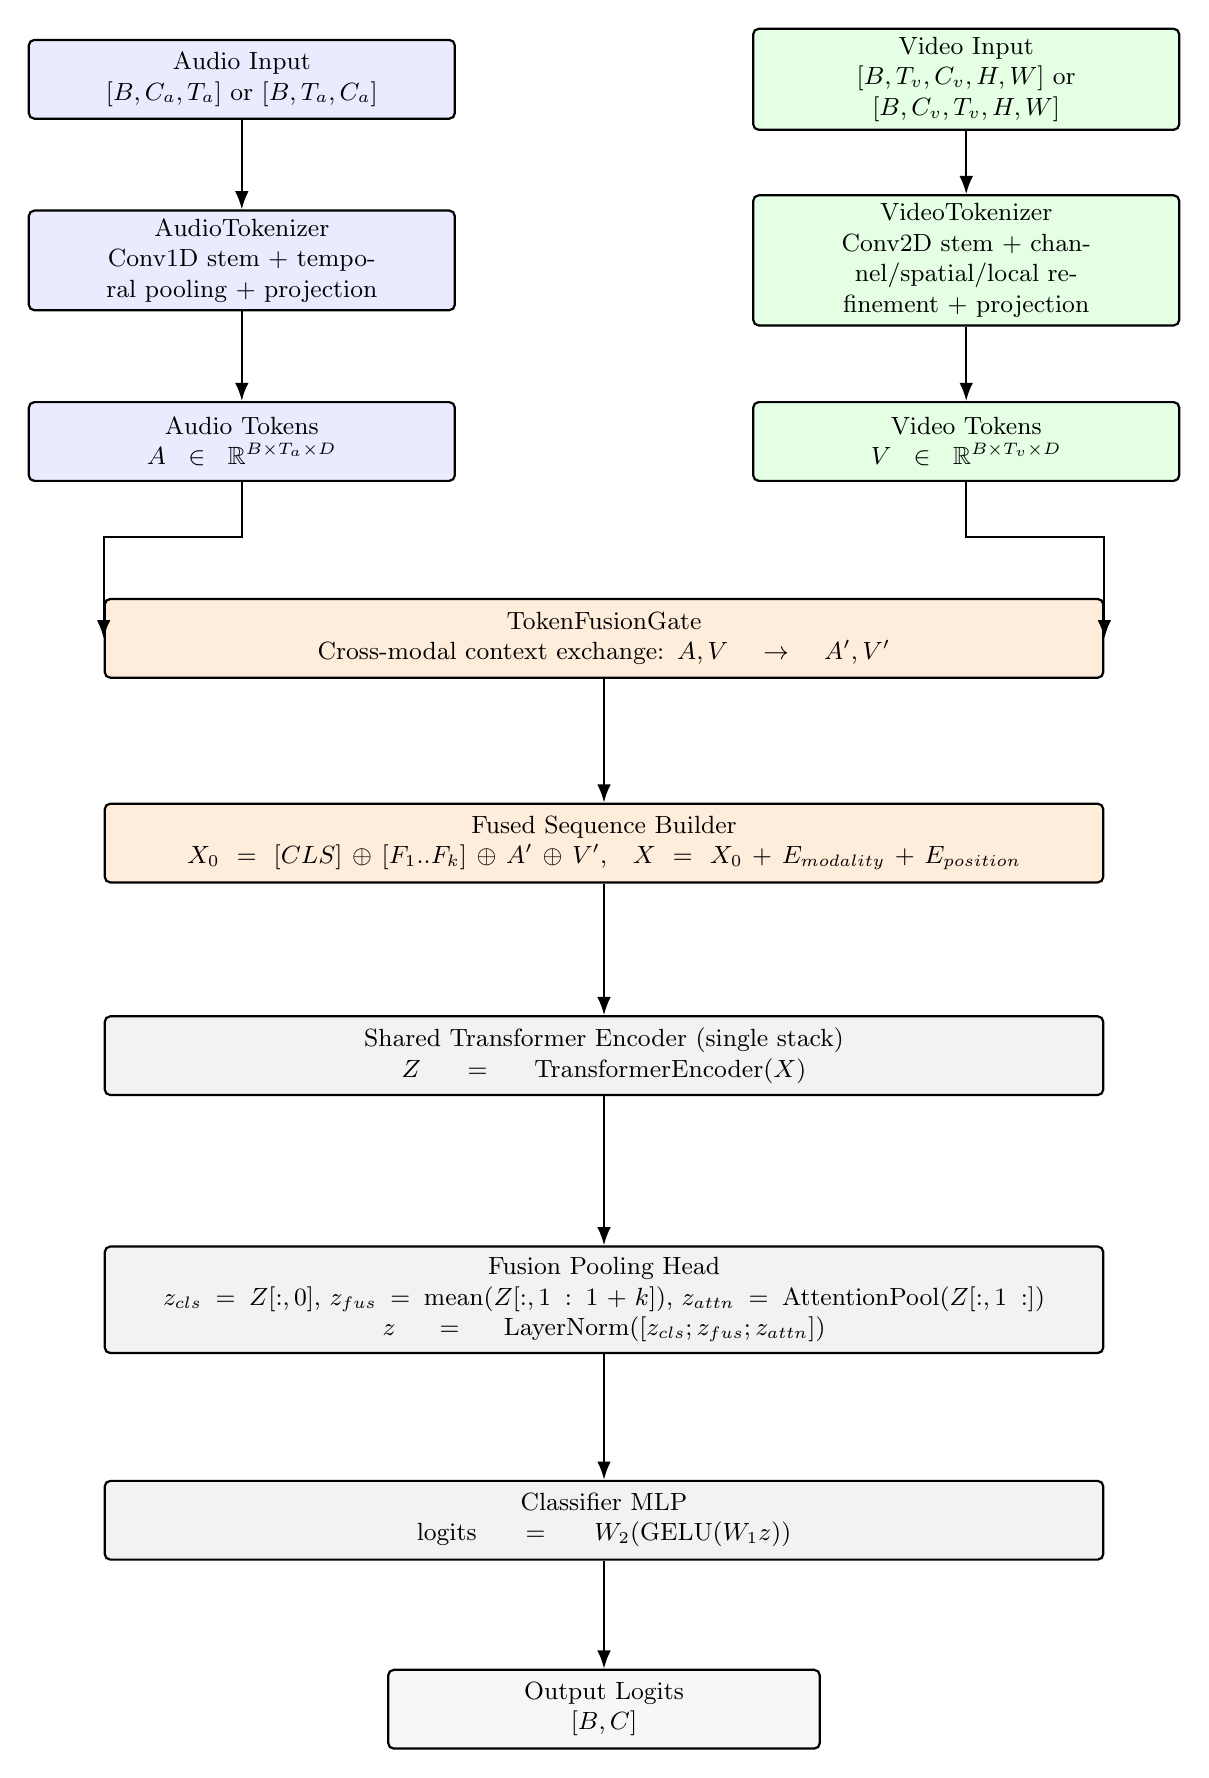
\begin{tikzpicture}[
  >=Latex,
  font=\small,
  audio/.style={draw, rounded corners=2pt, thick, align=center, text width=52mm, minimum height=10mm, inner sep=3pt, fill=blue!8},
  video/.style={draw, rounded corners=2pt, thick, align=center, text width=52mm, minimum height=10mm, inner sep=3pt, fill=green!10},
  fusion/.style={draw, rounded corners=2pt, thick, align=center, text width=124mm, minimum height=10mm, inner sep=4pt, fill=orange!14},
  shared/.style={draw, rounded corners=2pt, thick, align=center, text width=124mm, minimum height=10mm, inner sep=4pt, fill=gray!10},
  arr/.style={->, thick}
]
\node[audio] (audio_in) at (0,0) {Audio Input\\$[B,C_a,T_a]$ or $[B,T_a,C_a]$};
\node[video] (video_in) at (9.2,0) {Video Input\\$[B,T_v,C_v,H,W]$ or $[B,C_v,T_v,H,W]$};

\node[audio] (audio_tok) at (0,-2.3) {AudioTokenizer\\Conv1D stem + temporal pooling + projection};
\node[video] (video_tok) at (9.2,-2.3) {VideoTokenizer\\Conv2D stem + channel/spatial/local refinement + projection};

\node[audio] (audio_tokens) at (0,-4.6) {Audio Tokens\\$A \in \mathbb{R}^{B \times T_a \times D}$};
\node[video] (video_tokens) at (9.2,-4.6) {Video Tokens\\$V \in \mathbb{R}^{B \times T_v \times D}$};

\node[fusion] (gate) at (4.6,-7.1) {TokenFusionGate\\Cross-modal context exchange: $A,V \rightarrow A',V'$};
\node[fusion] (seq) at (4.6,-9.7) {Fused Sequence Builder\\$X_0=[CLS]\oplus[F_1..F_k]\oplus A'\oplus V'$,\quad $X=X_0+E_{modality}+E_{position}$};
\node[shared] (enc) at (4.6,-12.4) {Shared Transformer Encoder (single stack)\\$Z=\mathrm{TransformerEncoder}(X)$};
\node[shared] (pool) at (4.6,-15.5) {Fusion Pooling Head\\$z_{cls}=Z[:,0]$, $z_{fus}=\mathrm{mean}(Z[:,1:1+k])$, $z_{attn}=\mathrm{AttentionPool}(Z[:,1:])$\\$z=\mathrm{LayerNorm}([z_{cls};z_{fus};z_{attn}])$};
\node[shared] (clf) at (4.6,-18.3) {Classifier MLP\\$\mathrm{logits}=W_2(\mathrm{GELU}(W_1 z))$};
\node[shared, text width=52mm, fill=gray!6] (logits) at (4.6,-20.7) {Output Logits\\$[B,C]$};

\draw[arr] (audio_in) -- (audio_tok);
\draw[arr] (audio_tok) -- (audio_tokens);
\draw[arr] (video_in) -- (video_tok);
\draw[arr] (video_tok) -- (video_tokens);
\draw[arr] (audio_tokens.south) -- ++(0,-0.7) -| (gate.west);
\draw[arr] (video_tokens.south) -- ++(0,-0.7) -| (gate.east);
\draw[arr] (gate) -- (seq);
\draw[arr] (seq) -- (enc);
\draw[arr] (enc) -- (pool);
\draw[arr] (pool) -- (clf);
\draw[arr] (clf) -- (logits);
\end{tikzpicture}
\caption{TokenFusionAVTCA vertical architecture diagram. Blue: audio path, green: video path, orange: fusion stages, gray: shared backbone and head.}
\end{figure}

\subsection{Algorithm Design (Forward Pass)}
\begin{table}[H]
\centering
\begin{tabular}{p{0.97\linewidth}}
\toprule
\texttt{Algorithm TokenFusionAVTCA\_Forward(audio, video)} \\
\texttt{1. A <- AudioTokenizer(audio)} \\
\texttt{2. V <- VideoTokenizer(video)} \\
\texttt{3. (A, V) <- TokenFusionGate(A, V)} \\
\texttt{4. X <- concat(CLS, FusionTokens, A, V)} \\
\texttt{5. X <- X + ModalityEmbeddings + PositionalEmbeddings} \\
\texttt{6. Z <- SharedTransformerEncoder(X)} \\
\texttt{7. z <- concat(Z[:,0], mean(FusionSlice(Z)), AttentionPool(TokenSlice(Z)))} \\
\texttt{8. logits <- MLP(LayerNorm(z))} \\
\texttt{9. return logits} \\
\bottomrule
\end{tabular}
\caption{Forward algorithm summary aligned to the implemented design.}
\end{table}

\section{Fine-Tuning Progress (Epochs 77--80)}
\subsection{Training Behavior}
Training remained nearly saturated in this late stage:
\begin{itemize}
  \item Epoch 77: Train macro F1 = 100.0000, weighted F1 = 100.0000.
  \item Epoch 78: Train macro F1 = 99.9512, weighted F1 = 99.9479.
  \item Epoch 79: Train macro F1 = 99.9022, weighted F1 = 99.8957.
  \item Epoch 80: Train macro F1 = 99.8778, weighted F1 = 99.8957.
\end{itemize}

The first batch each epoch shows high data-loading latency spikes, then stabilizes quickly. This is consistent with loader warm-up and worker startup effects.

\subsection{Validation Metrics}
\begin{table}[H]
\centering
\begin{tabular}{rrrr}
\toprule
Epoch & Accuracy (\%) & Macro F1 (\%) & Weighted F1 (\%) \\
\midrule
77 & 67.50 & 65.3641 & 66.5034 \\
78 & 65.83 & 63.7318 & 64.7622 \\
79 & 66.87 & 65.0609 & 66.1799 \\
80 & 65.62 & 63.6156 & 64.6382 \\
\bottomrule
\end{tabular}
\caption{Validation performance for epochs 77--80.}
\end{table}

Best of this reported window is \textbf{epoch 77} by macro F1 and accuracy.

\section{Best Validation Snapshot (Epoch 77)}
\subsection{Classification Report}
\begin{center}
\begin{tabular}{lrrrr}
\toprule
Class & Precision & Recall & F1-score & Support \\
\midrule
neutral   & 0.5385 & 0.4375 & 0.4828 & 32 \\
calm      & 0.6897 & 0.9375 & 0.7947 & 64 \\
happy     & 0.7400 & 0.5781 & 0.6491 & 64 \\
sad       & 0.4938 & 0.6250 & 0.5517 & 64 \\
angry     & 0.8125 & 0.8125 & 0.8125 & 64 \\
fearful   & 0.8182 & 0.5625 & 0.6667 & 64 \\
disgust   & 0.6186 & 0.9375 & 0.7453 & 64 \\
surprised & 0.8065 & 0.3906 & 0.5263 & 64 \\
\midrule
accuracy      & \multicolumn{3}{r}{0.6750} & 480 \\
macro avg     & 0.6897 & 0.6602 & 0.6536 & 480 \\
weighted avg  & 0.6998 & 0.6750 & 0.6650 & 480 \\
\bottomrule
\end{tabular}
\end{center}

\subsection{Confusion Matrix (Epoch 77)}
\begin{table}[H]
\centering
\small
\begin{tabular}{lrrrrrrrr}
\toprule
True / Pred. & Neu & Cal & Hap & Sad & Ang & Fea & Dis & Sur \\
\midrule
Neutral   & 14 & 8 & 4 & 0 & 0 & 0 & 6 & 0 \\
Calm      & 0 & 60 & 0 & 4 & 0 & 0 & 0 & 0 \\
Happy     & 0 & 2 & 37 & 13 & 2 & 2 & 6 & 2 \\
Sad       & 10 & 6 & 0 & 40 & 2 & 2 & 4 & 0 \\
Angry     & 0 & 0 & 4 & 0 & 52 & 0 & 8 & 0 \\
Fearful   & 2 & 2 & 0 & 14 & 0 & 36 & 6 & 4 \\
Disgust   & 0 & 2 & 0 & 2 & 0 & 0 & 60 & 0 \\
Surprised & 0 & 7 & 5 & 8 & 8 & 4 & 7 & 25 \\
\bottomrule
\end{tabular}
\caption{Validation confusion matrix at epoch 77.}
\end{table}

\section{Improvement vs Previous Model}
Reference previous model outcome (from earlier run summary):
\begin{itemize}
  \item Accuracy: 0.2833
  \item Macro F1: 0.2086
  \item Weighted F1: 0.2226
\end{itemize}

Compared with current epoch-77 validation:
\begin{table}[H]
\centering
\begin{tabular}{lrrr}
\toprule
Metric & Previous & Current (Epoch 77 Val) & Absolute Gain \\
\midrule
Accuracy & 0.2833 & 0.6750 & +0.3917 \\
Macro F1 & 0.2086 & 0.6536 & +0.4450 \\
Weighted F1 & 0.2226 & 0.6650 & +0.4424 \\
\bottomrule
\end{tabular}
\caption{Overall metric improvement versus the earlier reported model output.}
\end{table}

Class-level F1 improvements are substantial for previously collapsed classes:
\begin{itemize}
  \item \textbf{neutral}: 0.0000 \(\rightarrow\) 0.4828
  \item \textbf{disgust}: 0.0000 \(\rightarrow\) 0.7453
  \item \textbf{surprised}: 0.0339 \(\rightarrow\) 0.5263
  \item \textbf{happy}: 0.1905 \(\rightarrow\) 0.6491
  \item \textbf{fearful}: 0.2222 \(\rightarrow\) 0.6667
\end{itemize}

\section{Interpretation}
\begin{itemize}
  \item The redesign clearly improved multimodal discrimination and reduced collapse into dominant classes.
  \item Late-stage training is almost saturated on train metrics (\(\sim 100\%\) macro F1), while validation remains around \(64\%{-}65\%\) macro F1, indicating a nontrivial generalization gap.
  \item Validation across epochs 77--80 is stable but fluctuates by about 1.7 macro-F1 points; checkpoint selection by macro F1 remains appropriate.
  \item Repeated \texttt{TypedStorage} warnings come from the image-to-tensor conversion path and are deprecation warnings, not correctness failures.
\end{itemize}

\section{Conclusion}
The fine-tuned \texttt{TokenFusionAVTCA} process has materially improved performance relative to the prior model behavior, especially on classes that previously had near-zero recall/F1. Based on the provided logs, epoch 77 is the strongest checkpoint in this window (\(67.5\%\) accuracy, \(65.36\%\) macro F1, \(66.50\%\) weighted F1 on validation).

For final model selection, the next formal step is to run and document a held-out test evaluation for the best-validation checkpoint using the same reporting protocol.

\end{document}
